\documentclass{article}

%Librerías
\usepackage[utf8]{inputenc}
\usepackage[spanish,mexico]{babel}
\usepackage{apacite}
\usepackage{pgfgantt}
\usepackage{pgfcalendar}


\bibliographystyle{apacite}
\setlength{\textwidth}{18cm}
\setlength{\oddsidemargin}{-1cm}
\setlength{\headsep}{-1cm}
\setlength{\voffset}{0cm}
\setlength{\topmargin}{0cm}
\setlength{\headheight}{0cm}

\usepackage{tikz}
\usepackage{multicol}
\usepackage{lipsum} 
%\bibliographystyle{apacite}
\usepackage[spanish]{babel}
\selectlanguage{spanish}


\begin{document}

%%%%%% ENCABEZADO %%%%%%%%%%%%%%%%%%%%%%%%%%%%%%%%%%%%%%%
% Logo de la maestría
\colorbox{white!10!}{
    \begin{minipage}[t]{0.05\textwidth} %0.165 
       \begin{flushright}
        
\includegraphics[width=2in]{logo UPS.png}
       \end{flushright}
    \end{minipage}
    \begin{minipage}[H]{0.62 \textwidth} %0.62
        \begin{center}
         
        \end{center}
     \end{minipage}
    \begin{minipage}[t]{0.05 \textwidth}
        \begin{flushleft}
        \hspace{10.25cm}
            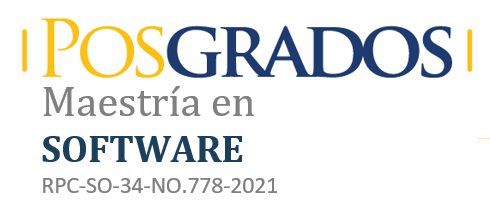
\includegraphics[width=2in]{Posgrados.png}
        \end{flushleft}
    \end{minipage}
}

\begin{tikzpicture}
    \draw[thick] (-6.5,0)--(11.2,0);
\end{tikzpicture}
%%%%%%%%%%%%%%%%%%%%%%%%%%%%%%%%%%%%%%%%%%%%%%%%%%%%%%%%%
\vspace{0.1cm}
\begin{center}
{\large\textsc{ANTEPROYECTO DEL TRABAJO DE TITULACIÓN}} \\
\vspace{0.5cm}
{ \large \textbf{Bryam Fernando Cabrera}} \\ 
\vspace{0.25cm}
{ \large \textbf{Willian Ariolfo  Lituma}}
\end{center}
\vspace{0.1cm}

\section{Tema del Trabajo de Titulación:  }
\begin{center}
Análisis, Desarrollo y Migración a un nuevo sistema contable para la empresa Accescont 
\end{center}
\section{Docente tutor propuesto:   }
\begin{center}
Asignar Tutor
\end{center}
\section{Antecedentes}

En el actual entorno empresarial, la tecnología de la información y los sistemas contables desempeñan un papel fundamental en el éxito y la eficiencia de las organizaciones. En este contexto, Accescont, una destacada firma de auditoría financiera con sede en Cuenca, Ecuador, se enfrenta a desafíos significativos debido a las limitaciones y obsolescencia de su sistema contable actual. Este sistema ha quedado rezagado en términos de funcionalidades y seguridad, lo que dificulta su capacidad para adaptarse a las crecientes necesidades de la empresa y la incorporación de nuevos módulos contables.

El principal problema de este sistema es su arquitectura monolítica, que ha sido objeto de modificaciones a lo largo de los años para satisfacer las necesidades cambiantes de la empresa. Sin embargo, estas modificaciones han llevado a una degradación significativa del código, lo que podría comprometer el sistema en caso de necesitar más cambios. En consecuencia, la empresa se ha visto en la necesidad de implementar un nuevo sistema de manera ágil, sin afectar a sus clientes.

El proyecto propuesto tiene como objetivo encontrar una solución integral y efectiva para fortalecer las operaciones contables de Accescont, especialmente en los módulos de clientes y proveedores. Esto se logrará mediante la implementación de nuevas herramientas, como los microservicios, que optimizarán la gestión financiera y contribuirán al crecimiento sostenible de la empresa. Además, este enfoque permitirá el escalado del sistema contable y posibles ampliaciones a otros módulos del sistema.

Es importante destacar que el éxito de este proyecto de titulación depende en gran medida del trabajo colaborativo con los usuarios y las partes interesadas de Accescont, así como del cumplimiento de plazos y la ejecución efectiva de las fases planificadas. \cite{Smith2023}

 %\lipsum[1-1]
       
 \section*{\textbf{Justificación del Tema de Trabajo de Titulación}}

 \begin{enumerate}
     \item \textbf{Contexto y Relevancia:} En el contexto empresarial actual, la tecnología de la información y los sistemas contables desempeñan un papel crítico para el éxito y la eficiencia de las organizaciones. Accescont, una firma de auditoría financiera con más de 35 años de experiencia con sede en Cuenca, Ecuador, se enfrenta a desafíos significativos debido a las limitaciones y la obsolescencia de su sistema contable actual. Este sistema, que ha sido parte integral de la empresa durante años, ha quedado rezagado en términos de funcionalidad y seguridad, lo que dificulta su capacidad para adaptarse a las cambiantes necesidades empresariales y la incorporación de nuevos módulos contables.
 
     \item \textbf{Problema de la Arquitectura Monolítica:} El principal problema radica en la arquitectura monolítica del sistema actual, que ha experimentado modificaciones a lo largo del tiempo para satisfacer las necesidades cambiantes de la empresa. Sin embargo, estas modificaciones han llevado a una degradación significativa del código, lo que podría comprometer aún más el sistema en caso de necesitar más cambios. Como resultado, la empresa reconoce la necesidad urgente de implementar un nuevo sistema contable sin afectar a sus clientes existentes.
 
     \item \textbf{Objetivos del Proyecto:} El proyecto propuesto se enmarca en la búsqueda de una solución integral y efectiva para fortalecer las operaciones contables de Accescont, especialmente en los módulos de clientes y proveedores. Se busca superar los desafíos tecnológicos actuales mediante la implementación de nuevas herramientas, como los microservicios, que optimizarán la gestión financiera y contribuirán al crecimiento sostenible de la empresa. Además, este enfoque permitirá el escalado del sistema contable y posibles expansiones a otros módulos del sistema.
 
     \item \textbf{Colaboración y Cumplimiento de Plazos:} Es importante destacar que el éxito de este proyecto de titulación dependerá en gran medida de la colaboración efectiva con los usuarios y las partes interesadas de Accescont. También se hará hincapié en el cumplimiento de los plazos y la ejecución eficiente de las fases planificadas para garantizar la implementación exitosa del nuevo sistema.
 
 \end{enumerate}
 
 En resumen, este trabajo de titulación busca abordar una problemática real en el ámbito empresarial. Accescont se enfrenta a desafíos tecnológicos y de usabilidad con su sistema contable actual, y el proyecto propuesto tiene como objetivo superar estos desafíos mediante la implementación de una solución innovadora y escalable. La colaboración con los stakeholders y el cumplimiento de los plazos son elementos clave para el éxito de este proyecto y su contribución al crecimiento y competitividad de Accescont en el mercado. 

\section{Objetivos:}

\subsection{Objetivo General}

Analizar, desarrollar y migrar los módulos de clientes y proveedores del sistema contable de la empresa Accescont en la ciudad de Cuenca, reemplazando su sistema actual por uno de naturaleza modular con el propósito de mejorar la escalabilidad.

\subsection{Objetivos Específicos}

\begin{enumerate}
    \item Analizar los requerimientos para los módulos del nuevo sistema contable con la participación de los usuarios y partes interesadas, aplicando la metodología SCRUM y posteriormente desarrollar un sistema contable ajustado a las necesidades detectadas en los requerimientos.
    
    \item Planificar el desarrollo de los módulos en etapas, para controlar el avance del proyecto y cumplir con los tiempos establecidos en el cronograma.
    
    \item Desarrollar los módulos de clientes y proveedores para el sistema contable que cumpla con los requisitos identificados, usando metodologías ágiles de desarrollo de software con el propósito de acoplarlos con otras funcionalidades que tendría el sistema completo.
    
    \item Realizar pruebas para garantizar la calidad y funcionalidad de los módulos desarrollados, usando pruebas de validación y criterios de aceptación, para asegurar que el sistema funcione acorde a las necesidades de las partes interesadas.
\end{enumerate}


\section{Alcance:}
El proyecto consiste en Analizar, desarrollar y migrar los módulos de clientes y proveedores del sistema contable de la empresa Accescont de la ciudad de Cuenca, que luego de las pruebas y validaciones necesarias sea implementado en conjunto los demás módulos planeados para el sistema contable de la empresa. Por lo antes expuesto este proyecto únicamente cubrirá los módulos de clientes y proveedores para los cuales se hará una revisión e identificación de requisitos, construcción, migración de datos, pruebas y evaluación.

\section{Metodología}

En esta sección se describe la metodología que se seguirá para lograr los objetivos específicos del proyecto. Se detalla cómo se abordarán cada uno de los objetivos para alcanzar el objetivo general.

\begin{figure}[h]
    \centering
    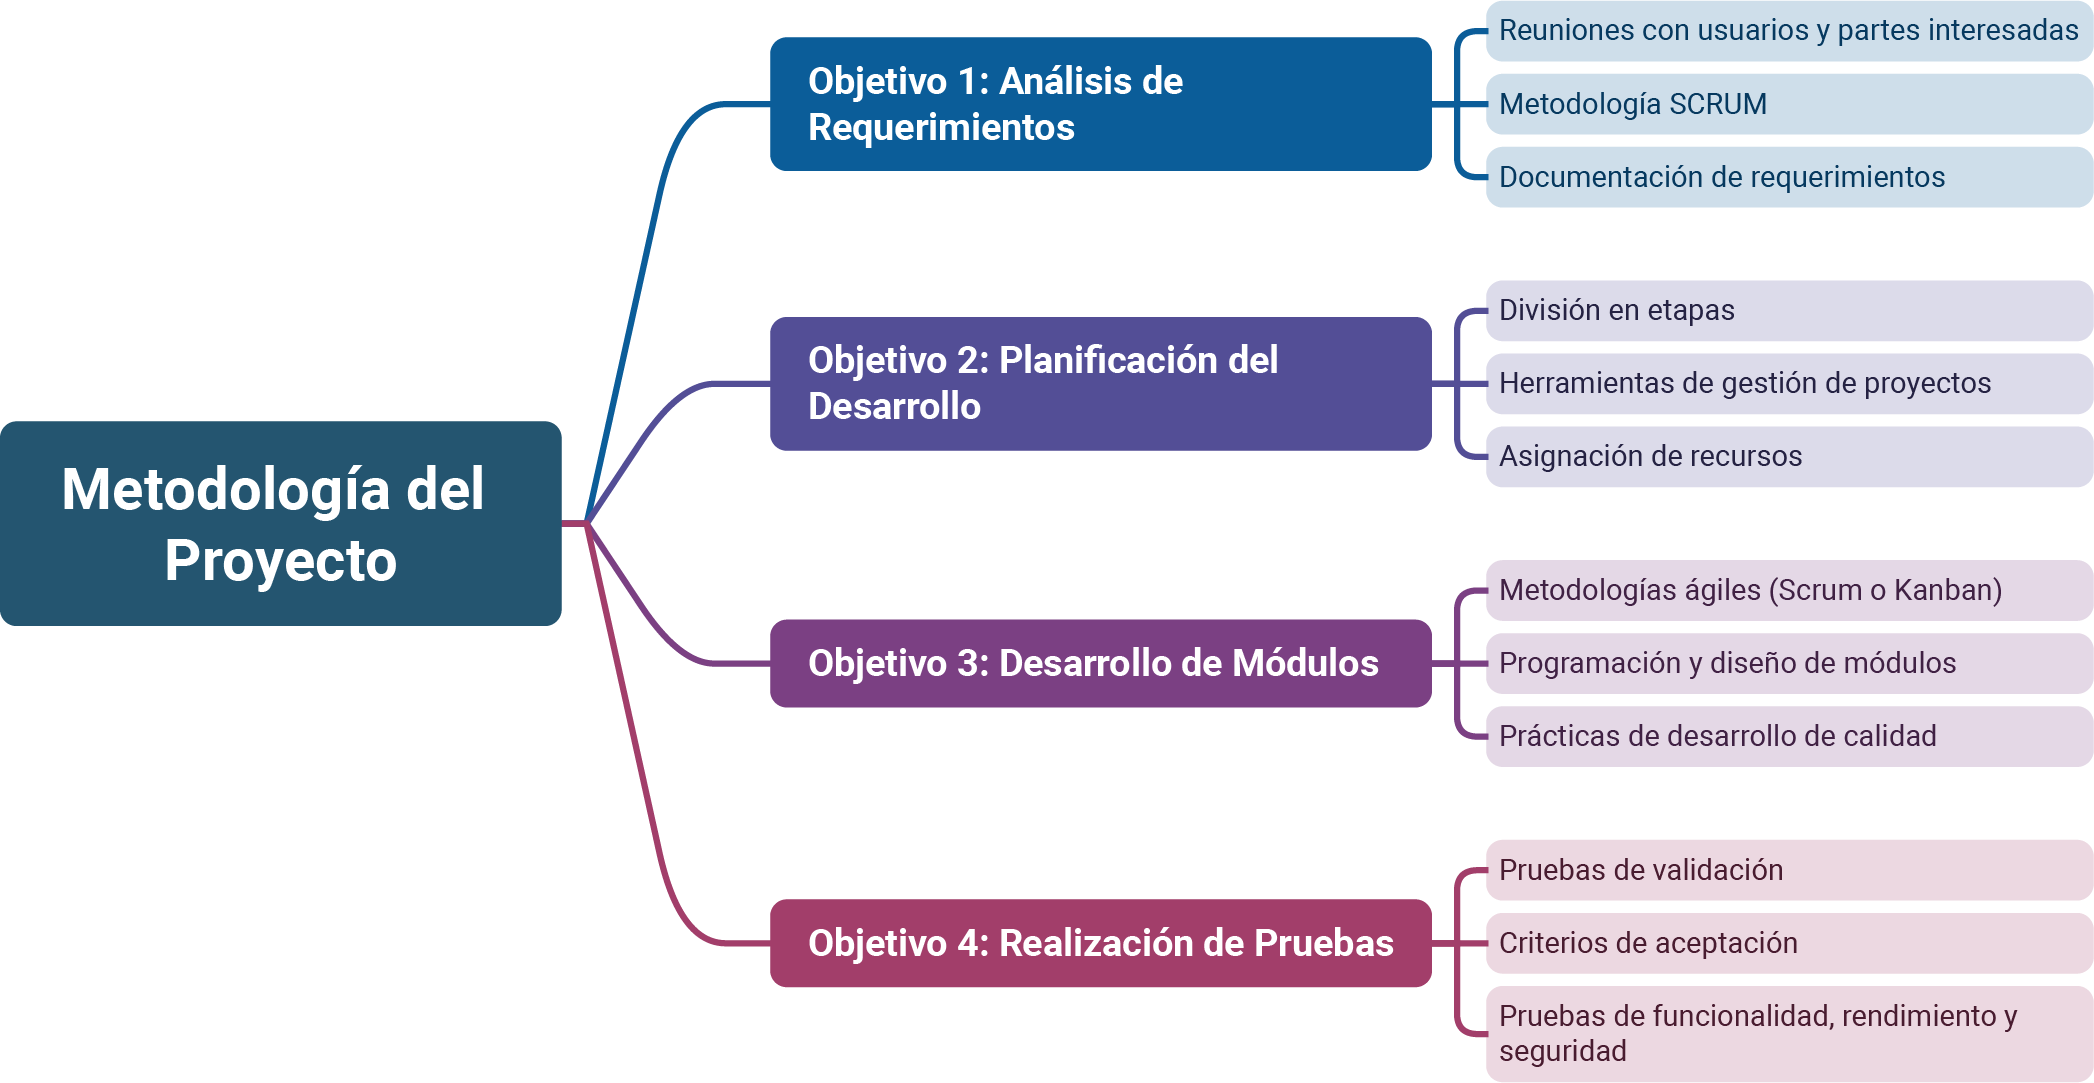
\includegraphics[width=0.8\textwidth]{med.png}
    \caption{Diagrama de flujo del análisis de requerimientos.}
\end{figure}

\subsection{Objetivo 1: Análisis de requerimientos}

Para lograr el primer objetivo específico, que consiste en analizar los requerimientos para los módulos del nuevo sistema contable, se seguirá la metodología siguiente:

\begin{itemize}
    \item Se llevarán a cabo reuniones con los usuarios y partes interesadas de Accescont para recopilar información detallada sobre los requerimientos.
    \item Se utilizará la metodología SCRUM para facilitar la comunicación con los stakeholders y garantizar una comprensión clara de sus necesidades.
    \item Se documentarán los requerimientos identificados en un documento formal que servirá como base para el desarrollo.
\end{itemize}

\subsection{Objetivo 2: Planificación del desarrollo}

Para alcanzar el segundo objetivo específico, que implica la planificación del desarrollo de los módulos, se aplicarán los siguientes pasos:

\begin{itemize}
    \item Se dividirá el desarrollo en etapas claras y manejables, definiendo hitos y entregables para cada una.
    \item Se utilizarán herramientas de gestión de proyectos para controlar el avance del proyecto y asegurarse de que se cumplan los tiempos establecidos en el cronograma.
    \item Se asignarán recursos adecuados a cada etapa, incluyendo personal, tiempo y tecnología.
\end{itemize}

\subsection{Objetivo 3: Desarrollo de módulos}

Para lograr el tercer objetivo específico, que se refiere al desarrollo de los módulos de clientes y proveedores, se seguirán los siguientes pasos:

\begin{itemize}
    \item Se utilizarán metodologías ágiles de desarrollo de software, como Scrum o Kanban, para garantizar la flexibilidad y adaptabilidad durante el proceso de desarrollo.
    \item Se programarán y diseñarán los módulos teniendo en cuenta los requerimientos identificados en el primer objetivo específico.
    \item Se utilizarán prácticas de desarrollo de software de alta calidad para garantizar la funcionalidad y la eficiencia de los módulos.
\end{itemize}

\subsection{Objetivo 4: Realización de pruebas}

Para alcanzar el cuarto objetivo específico, que consiste en realizar pruebas de calidad, se llevarán a cabo las siguientes actividades:

\begin{itemize}
    \item Se ejecutarán pruebas de validación para asegurarse de que los módulos cumplan con los requerimientos especificados.
    \item Se establecerán criterios de aceptación que definan cuándo un módulo se considera completado y funcional.
    \item Se realizarán pruebas exhaustivas de funcionalidad, rendimiento y seguridad para garantizar la calidad del sistema.
\end{itemize}
\section{Cronograma de Actividades}

En esta sección se presenta el cronograma de actividades planificado para el desarrollo del proyecto. El cronograma detalla las tareas a realizar, los responsables de cada tarea y las fechas de inicio y finalización.

\begin{ganttchart}[
    hgrid,
    vgrid,
    x unit=0.07cm, % Ajusta este valor según tu preferencia
    time slot format=isodate,
    time slot unit=day,
    vrule/.style={red, dashed, thick},
    vrule label font=\bfseries\small,
    title height=1, % Altura del título
    title label font=\bfseries\small,
    group height=0.7, % Altura de las barras
    group label font=\bfseries\small,
    group label node/.append style={align=right},
    bar height=0.4, % Altura de las tareas
    bar label font=\small,
    milestone height=0.8, % Altura de los hitos
    milestone label font=\small,
    bar top shift=0.2, % Ajusta la posición vertical de las tareas
    bar/.append style={draw=none, fill=blue!90}, % Estilo de las barras
    milestone/.append style={draw=none, fill=red}, % Estilo de los hitos
    ]{2023-10-01}{2024-03-31}
    
    % Cambia las fechas a semanas
    \gantttitlecalendar{year, month=week} \\
    
    \ganttbar{Reuniones iniciales}{2023-10-01}{2023-10-07} \\
    \ganttbar{Análisis de requerimientos}{2023-10-08}{2023-10-14} \\
    \ganttbar{Planificación del desarrollo}{2023-10-15}{2023-10-21} \\
    \ganttbar{Desarrollo de módulos}{2023-10-22}{2023-10-28} \\
    \ganttbar{Pruebas de validación}{2023-10-29}{2023-11-04} \\
    \ganttbar{Pruebas de rendimiento}{2023-11-05}{2023-11-11} \\
    \ganttbar{Evaluación final}{2023-11-12}{2023-11-18} \\
    \ganttbar{Documentación final}{2023-11-19}{2023-11-25} \\
    \ganttbar{Presentación del proyecto}{2023-11-26}{2023-12-02} \\
    \ganttnewline[thick, blue]
    
    \ganttbar{Reuniones semanales}{2023-10-01}{2023-12-02} \\
    \ganttbar{Revisión intermedia}{2023-11-12}{2023-11-18} \\
    \ganttbar{Presentación final}{2023-12-01}{2024-03-31} \\
\end{ganttchart}

\section{Presupuesto: (Opcional)}

Este apartado incluirá los recursos e información financiera para el Trabajo de Titulación. 
%\bibliographystyle{abbrv}
%apacite



\bibliography{sample}

\vspace{1cm}
Este apartado contiene el listado de referencias empleadas para la elaboración del documento, de preferencia en formato APA u otros formatos Preconocidos.


\end{document}
